\documentclass{article}
\usepackage{graphicx}
\usepackage{tcolorbox}
\usepackage{framed}
\usepackage{array}
\usepackage{multirow}
\usepackage{tabularx}

\usepackage{booktabs}

\usepackage{hyperref}
\hypersetup{
    colorlinks=true,
    linkcolor=green,
    filecolor=magenta,      
    urlcolor=cyan,
}

\usepackage[letterpaper, margin=2in]{geometry}
\geometry{
 legalpaper,
 total={210mm,297mm},
 left=20mm,
 right=20mm,
 top=20mm,
 bottom=20mm,
 }

\newcommand{\specialcell}[2][c]{%
  \begin{tabular}[#1]{@{}c@{}}#2\end{tabular}}

\author{Vaibhav}
\begin{document}

%----------------------------------------------------------------------------------------------------------------------%%
%                                                  Header
	\begin{tabular}{lc l r}
		\begin{minipage}{0.8\textwidth}
			\begin{flushleft}
				\large{\textbf{KUMBHAR VAIBHAV ANANDA}}\\
				 \vspace{0.5cm}
				\begin{tabular}{lcl}
				Mobile No & : & +91-9403183440\\
				 \vspace{0.5cm}
				Email-Id & : & \href{mailto:vkumbhar94@gmail.com}{vkumbhar94@gmail.com}
				\end{tabular}
			\end{flushleft}
		\end{minipage}
		&
		\begin{minipage}{0.2\textwidth}
			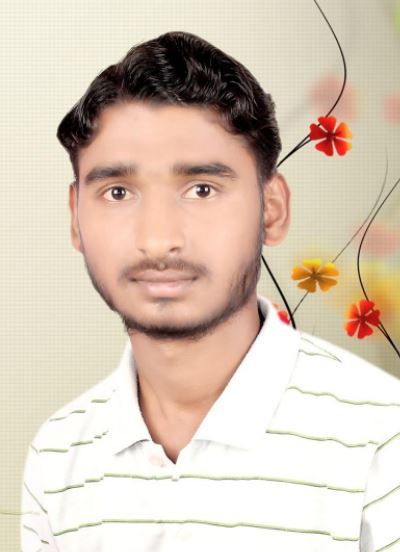
\includegraphics[width=0.8\textwidth]{A.jpg}
		\end{minipage}
	\end{tabular}\\
\\

%----------------------------------------------------------------------------------------------------------------%%%
%                                        Career objective
%\begin{tcolorbox}
\begin{framed}
	\large{\textbf{CAREER OBJECTIVE}}
\end{framed}
%\end{tcolorbox}
	\large{\textup{To work in an environment of growth and excellence and utilize my skills to achieve personal as well as organizational goals.}}


%--------------------------------------------------------------------------------------------------------------------------
%                                    Personal Details
\begin{framed}
	\large{\textbf{PERSONAL DETAILS}}
\end{framed}
\begin{tabular}{lcm{0.5\linewidth}}
	\textbf{Local Address} & : & Flat No: 11, Silver Oak Park, MSEB Road, Vishrambag, Sangli-416415\\
	\textbf{Permanent Address} & : & A/P: - Marawade, Tal: - Mangalwedha, Solapur- 413319\\
	\textbf{Languages known} & : &  English, Hindi, \underline{\textbf{Marathi}}.
\end{tabular}

%---------------------------------------------------------------------------------------------------------------------------
%                                      Engineering Qualification

\begin{framed}
	\large{\textbf{ENGINEERING QUALIFICATION}}
\end{framed}
\large{\textbf{Branch: Computer Science and Engineering}}

\begin{flushleft}

\setlength{\tabcolsep}{0.7em}
\def\arraystretch{1.7}
\begin{tabular}{|p{\dimexpr.19\textwidth} |>{\centering\arraybackslash} p{\dimexpr.33\textwidth-3\tabcolsep} |p{\dimexpr.19\textwidth-3\tabcolsep} |
		p{\dimexpr.16\textwidth-3\tabcolsep} | p{\dimexpr.16\textwidth-3\tabcolsep}|}
	\hline
	\centering\textbf{CLASS} & \centering\textbf{INSTITUTE} & \centering\textbf{SEM-I} & \centering\textbf{SEM-II} & \textbf{YEAR}\\
	\hline
	\centering Third Year &  \multirow{3}{*}{ \specialcell{Walchand College \\ Of Engineering, Sangli}} & \centering 8.21 & \centering Pursuing & 2014-15\\
	\cline{1-1}\cline{3-5}
	\centering Second Year&  & \centering 7.48 & \centering 7.52 &  2013-14 \\
	\cline{1-1}\cline{3-5}
	\centering First Year & & \centering  7.28 & \centering 7.38 & 2012-13 \\
	\hline
\end{tabular}
\end{flushleft}


%----------------------------------------------------------------------------------------------------------------------------------
%				Pre-Engineering Qualification
\begin{framed}
	\large{\textbf{PRE-ENGINEERING QUALIFICATION}}
\end{framed}
\begin{flushleft}
\setlength{\tabcolsep}{0.7em}
\def\arraystretch{1.7}
\begin{tabular}{|p{\dimexpr.17\textwidth} | p{\dimexpr.35\textwidth-3\tabcolsep} |p{\dimexpr.17\textwidth-3\tabcolsep} |
		p{\dimexpr.17\textwidth-3\tabcolsep} | p{\dimexpr.17\textwidth-3\tabcolsep}|}
	\hline
\centering\textbf{EXAM} & \centering\textbf{ INSTITUTE} & \centering\textbf{BOARD} & \centering\textbf{MARKS}& \textbf{YEAR}\\
	\hline
	\centering H.S.C. & \specialcell{  Karmveer Bhaurao Patil\\ Mahavidyalaya, Pandharpur}  & \multirow{2}{*}{ \specialcell{PUNE}} & \centering 83.33 & \specialcell{ 2011-12}\\
	\cline{1-2}\cline{4-5}
	\centering S.S.C. & \centering Hanuman Vidya Mandir, Marawade &  & \centering 91.45 & 2009-10 \\
	\hline
\end{tabular}
\end{flushleft}



%----------------------------------------------------------------------------------------------------------------------------------
%				Technical Skills
\begin{framed}
	\large{\textbf{TECHNICAL SKILLS}}
\end{framed}
\setlength{\tabcolsep}{0.7em}
\def\arraystretch{1.7}
\begin{tabular}{lcl}
	Languages & : & C, C++, Java, PL-SQL, Python (Novice)\\
	Operating System &  : &  Windows 8, Ubuntu- 13.04/14.10\\
	Development Tools &  : & IntelliJ Idea 14.0.1, Eclipse, Visual Studio 2013(Novice)\\
	Versioning Control Tools & : & Git\\
	Technologies &  : &  Django (Novice), Android (Novice)  
\end{tabular}

\newpage
%----------------------------------------------------------------------------------------------------------------------------------
%				Projects Undertaken
\begin{framed}
	\large{\textbf{PROJECTS UNDERTAKEN}}
\end{framed}
\setlength{\tabcolsep}{0.1em}
\def\arraystretch{1.7}
\begin{center}
\begin{tabularx}{\linewidth}{|X|X|X|X|X|}
	\hline
	\centering\textbf{YEAR} & \centering\textbf{ TITLE} & \centering\textbf{PROJECT TYPE} & \centering\textbf{DESCRIPTIOIN} & \textbf{TECHNOLOGY USED}\\
\hline

	\centering{ T.Y. B. Tech} & 
	\centering 
		\begin{itemize}
				\item A Context Awareness App
				\item Prototyping Augmented Reality Systems for Exploring the College campus using Android app.
		\end{itemize}
 	&
	\centering Mini Project&
	\centering Ease to get Information of College's All Departments, Labs and Library. 
	&
	\begin{itemize}
		\item Augmented Reality SDK
		\item Android
	\end{itemize}\\
	\hline
	
	\centering T.Y. B. Tech & 
	A Technical Forum  & Mini Project & Ease to solve technical Queries of students &
	\begin{itemize}	
		\item Django with Python
		\item Bootstrap
	\end{itemize} \\
	\hline
\end{tabularx}
\end{center}


%----------------------------------------------------------------------------------------------------------------------------------
%				WORKSHOP ATTENDED
\begin{framed}
	\large{\textbf{WORKSHOP ATTENDED}}
\end{framed}

\begin{itemize}
	\item Attended workshop on \textbf{"Hadoop Basics"} in March 2015 by "Mr. Kapil Bhosale".
	\item Attended workshop on \textbf{"Ruby on rails Workshop"} by Sushant Mane.
	\item Attended workshop on \textbf{"Clean Coding and Object Oriented Design"} by \textbf{"Thaughtworks"}. 
\end{itemize}



%----------------------------------------------------------------------------------------------------------------------------------
%				CO-CURRICULAR ACTIVITIES
\begin{framed}
	\large{\textbf{CO-CURRICULAR ACTIVITIES}}
\end{framed}
\begin{itemize}
	\item Winner in \textbf{"Code Marathon"} in \textbf{"Vision 2014"}.
	\item Runner up in \textbf{"Code Trix"}  by \textbf{ "SAIT Club"}.
\end{itemize}





%----------------------------------------------------------------------------------------------------------------------------------
%				EXTRA-CURRICULAR ACTIVITIES
\begin{framed}
	\large{\textbf{EXTRA-CURRICULAR ACTIVITIES}}
\end{framed}

\textbf{Association of Computer Science and Engineering Students (ACSES)}
\begin{itemize}	
	\item Appointed as \textbf{Program director} of \textbf{ACSES} a leading students’ organization in WCE, Sangli for the year 2014-2015.
	\item Organized Social Event \textbf{SITAC (Social IT Awareness Campaign)} by \textbf{ACSES} on “Computer Technology and Introduction to Computer”.
	\item Worked as \textbf{Coordinator} of \textbf{ACSES}, member of committee of \textbf{TECHUMEN 2k13}
	\item Contributed in \textbf{SITAC 2k13}
	
\end{itemize}

\newpage


%----------------------------------------------------------------------------------------------------------------------------------
%				HOBBIES
\begin{framed}
	\large{\textbf{HOBBIES}}
\end{framed}
\begin{itemize}
	\item Coding
	\item Learning New Technologies.
	\item Daily Workout.
	\item Listening Songs. 
\end{itemize}


%----------------------------------------------------------------------------------------------------------------------------------
%				DECLARATION
\begin{framed}
	\large{\textbf{DECLARATION}}
\end{framed}
	\Large{I hereby declare that all the information provided above is true to the best of my knowledge. }


\vspace{3cm}
\begin{tabular}{cc}
\begin{minipage}{0.5\textwidth}
\begin{flushleft}Place:
\end{flushleft}
\end{minipage}
&
\begin{minipage}{0.5\textwidth}
\begin{center}Signature:
\end{center}
\end{minipage}
\end{tabular}


\begin{tabular}{cc}
\begin{minipage}{0.5\textwidth}
\begin{flushleft}Date:
\end{flushleft}
\end{minipage}
&
\begin{minipage}{0.5\textwidth}
\begin{center} (Kumbhar Vaibhav A.)
\end{center}
\end{minipage}
\end{tabular}

\end{document}